

\chapter{Joint Executions}

\label{ch:jointexec}

This chapter constructs a new representation for the actions to be
performed by a team of agents during the cooperative execution of
a shared task. Dubbed \emph{joint executions}, they are partially-ordered
branching sequences of actions that allow independent actions to be
performed independently, while using each agent's local view to ensure
that synchronisation is always possible when required. Using these
structures, our MIndiGolog execution planner can produce plans suitable
for execution in asynchronous multi-agent domains.

The fundamental unit of reasoning in the situation calculus, and the
output of the standard Golog execution planning process, is the \emph{situation}:
a complete, ordered sequence of all actions that are to be performed.
This is suboptimal for representing plans in an asyncrhonous multi-agent
setting in three ways:

\begin{itemize}
\item it does not permit branching depending on information obtained at
run-time 
\item it enforces a strict execution order on actions that are potentially
independent, requiring inter-agent syncrhonisation when it is not
actually necessary 
\item it requires a strict execution order on actions that may be hidden
from some agents, demanding inter-agent synchronisation that is not
actually possible 
\end{itemize}
As we have demonstrated in Chapter \ref{ch:mindigolog}, restricting
the domain to be synchronous and completely known lets the agents
make effective use of raw situation terms for planning. But moving
to asynchronous domains with incomplete knowledge requires a more
powerful structure for representing the actions to be performed.

To build such a structure, we take inspiration from a model of concurrent
computation known as \emph{prime event} \emph{structures}, which are
partially-ordered branching sequences of events \citep{npw79event_structures}.
A \emph{joint execution} is defined as a particular kind of prime
event structure that is rich enough to capture the concurrent execution
of independent actions, and can branch on the sensing results of actions.
We use our explicit account of an agent's local view to identify joint
executions that can feasibly be executed based on the local infomation
available to each agent at runtime.

Joint executions are also formalised in a way that is easily translated
into an implementation. They can be built up one action at a time
in much the same way as ordinary situation terms. If the theory of
action meets some simple restrictions, joint executions can also be
reasoned about using standard regression techniques. We demonstrate
an implementation that performs offline execution planning for an
asyncrhonous, partially observable domain, and discuss the challenges
faced when moving to an online execution model.

These structures thus allow us to represent the actions that a team
of agents are to perform in service of some shared task, without requiring
constant synchronization between the agents, and without assuming
that agents know all the actions that have been performed, while utilizing
existing reasoning methods and planning machinery. This is a significant
increase in power over existing approaches to planning for multi-agent
teams in the situation calculus.

The chapter proceeds as follows: TODO.


\section{Background\label{sec:JointExec:Background}}

The above discussion highlights three desirable properties of a plan
representation formalism intended for use in asyncrhonous multi-agent
domains: it must be \emph{partially-ordered}, \emph{branching}, and
\emph{feasible}. While each of these aspects have been studied in
isolation in the situation calculus, our work is the first to combine
them into a single formalism suitable for a multi-agent setting.


\subsection{Partial Ordering}

There has been little work on partial-order planning in the situation
calculus, most likely because the use of situations heavily biases
the reasoning machinery towards totally-ordered sequences of actions.
While \citet{son00htn_golog} allow the programmer to specify partial-orders
on actions by adding operators to the Golog language, the actual plans
produced by their system are still raw situation terms. One exception
is \citep{plaisted97sc_aspect}, which extends the situation calculus
with explicit {}``aspects'' and allows partial ordering between
actions that affect different aspects of the world state. By contrast,
we seek to leverage the existing meta-theory of the standard situation
calculus.

Partial-order planning is the mainstay of the closely-related \emph{event
calculus} formalism. Here each action is specified to happen at a
specific time, and the constraints on relative occurrence times of
actions determine a partial ordering. \citet{Shanahan97ec_planning}
has shown that abductive theorem proving in the event calculate generates
partially-ordered plans, and the mechanics of the theorem prover naturally
mirror various concepts from the goal-based partial-order planning
literature, such as conflicts, threats and links \citep{peot92conditional_nonlinear}.

The close similarities between the situation and event calculi are
well understood, as are the advantages of the event calculus when
it comes to working with partially-ordered action sequences \citep{belleghem97sitcalc_evtcalc}.
Indeed, it is possible to implement a Golog interpreter on top of
the event calculus that naturally generates partially-ordered plans
\citep{pereira04ec_golog}. Perhaps we should simply adopt a formalism
such as the event calculus that is naturally partially-ordered, rather
than trying to construct partially-ordered representations on top
of the naturally sequential situation calculus?

While having a partial-order representation is important, it is not
the complete picture. We don't want the agents to have to synchronise
their actions unnecessarily, but we also need to ensure the converse:
that when an explicit ordering between actions is necessary, the required
synchronisation is actually possible based on the local information
available to each agent. It is not clear how techniques such as \citep{pereira04ec_golog}
would extend to the asynchronous multi-agent case.

As we shall see, the formalism we develop in this chapter enables
these dual requirements - that some actions don't need to be ordered,
while other actions must not be ordered - to be captured in quite
an elegant way without stepping outside the bounds of existing situation
calculus theory.


\subsection{Branching}

Several single-agent formalisms based on the situation calculus have
introduced some form of branching into the structures returned by
the planner, including the conditional action trees of of sGolog \citep{lakemeyer99golog_cats}
and the branching IndiGolog plans of \citep{giacomo04sem_delib_indigolog}.
These structures typically branch based on the truth or falsehood
of test conditions included in the program, rather than directly on
the sensing results returned by an action. For example, the definition
of conditional action trees in \citep{lakemeyer99golog_cats} includes
the following branching case:\[
c=[\phi,c_{1},c_{2}]\]


This instructs the agent to execute the sub-tree $c_{1}$ if $\phi$
is true and the sub-tree $c_{2}$ if $\phi$ is false. While this
works well for a single agent, it is not clear how to extend it to
cooperative execution in a multi-agent setting, where some members
of the team may not know whether or not $\phi$ holds.


\subsection{Feasibility\label{sec:JointExec:BG:Feasibility}}

To allow an agent to execute a plan that depends on information collected
at run-time, it is not sufficient to simply introduce branching into
the plan representation formalism. One must also ensure that, at execution
time, the agent will always \emph{know} which branch of the plan to
take. For example, suppose this simple branching plan will provably
achieve a goal:\[
\mathbf{if}\,\,\phi\,\,\mathbf{then}\,\, action_{1}\,\,\mathbf{else\,}\, action_{2}\]


The agent can only execute this program if it knows whether or not
$\phi$ holds; otherwise, although one of the branches is guaranteed
to achieve the goal, the agent does not know which branch to take.
Feasibility is typically guaranteed by including sensing actions to
ensure that the test conditions become known when needed:\[
sense_{\phi}\,\,;\,\mathbf{if\,}\,\phi\,\,\mathbf{then}\,\, action_{1}\,\,\mathbf{else\,}\, action_{2}\]


This requirement that an agent {}``knows how'' to execute a plan
is formalised by various notions of \emph{epistemic feasibility},
including those of \citep{levesque98what_robots_can_do,levesque00knowing_how,Lesperance01epi_feas_casl,giacomo04sem_delib_indigolog,baier06programs_that_sense}.

One approach to ensuring feasibility, embodied by \citep{levesque00knowing_how,giacomo04sem_delib_indigolog,baier06programs_that_sense},
is to represent plans by arbitrary programs formulated in a control
language such as Golog. One then semantically characterises the class
of epistemically feasible programs, using direct assertions about
the knowledge of each agent at each stage of execution. While this
allows for potentially very rich, very succinct plans, it is not clear
how to systematically generate an epistmically feasible plan using
such a general characterisation.

Another approach, advocated by \citep{levesque96what_is_planning,levesque98what_robots_can_do}
and used in the implementation section of \citep{giacomo04sem_delib_indigolog},
is to restrict the structure of plans so that they are always epistemically
feasible. For example, the {}``robot programs'' of \citep{levesque98what_robots_can_do}
are restricted to simple operators such as:\begin{gather*}
action\\
seq(\delta_{1},\delta_{2})\\
branch(action,\delta_{1},\delta_{2})\\
loop(branch(action,\delta,exit))\end{gather*}


These programs do not contain test conditions, but rather branch directly
on the (binary) sensing results returned from each action. There is
therefore no potential for confusion when executing such programs;
they are essentially equivalent to a kind of finite automaton that
can be executed reactively. Nevertheless, \citet{levesque98what_robots_can_do}
show that these programs are universal, in the sense that any achievable
goal can be achieved by suitable a robot program. We are not aware
of any work extending this approach to represent programs to be exeuted
cooperatively by a team of agents.

These existing notions of epistemic feasibility can be characterised
as \emph{knowing what}. At each stage of execution, each agent must
know what its next action is. In synchronous domains with public actions,
as typically studied in the situation calculus, this is sufficient
to ensure the feasibility of executing a plan.

In asynchronous domains it is not enough for an agent to know \emph{what}
its next action is; it must also know \emph{when} that action should
be performed. For example, suppose that the following simple plan
provably achieves a goal:\[
action_{1}(agt_{1})\,;\, action_{2}(agt_{2})\]


In a synchrononous domain this plan can be executed directly. But
suppose the domain is asynchronous, and $agt_{2}$ is unable to observe
the occurrence of $action_{1}$. Since $agt_{2}$ has no way of knowing
whether or not $action_{1}$ has been performed yet, it will not know
when to perform $action_{2}$ and the plan cannot be executed.

In this chapter we ensure plan feasibility by restricting the structure
used to represent plans, in an approach similar to \citep{levesque98what_robots_can_do}
but without looping constructs. We use the explicit account of each
agent's local view developed in the previous chapter to ensure that
each agent will always have enough information to determine what action
to perform next, and when to perform it.


\subsection{Event Structures}

To tackle cooperative execution in a multi-agent setting, we have
adopted a model of concurrent computation known as \emph{event structures}
\citep{npw79event_structures}. The particular variant we are interested
in are \emph{prime event structures}, canonically defined as a four-tuple
as follows.

\begin{defnL}
[{Prime~Event~Structure}] A prime event structure is a
four-tuple $(\mathcal{V},\gamma,\prec,\oplus)$ where: $\mathcal{V}$
is a set of events; $\gamma$ is a function assigning a label to each
event; $\prec$ is the precedence relation, a strict partial order
on events; $\oplus$ is the conflict relation, a binary symmetric
relation indicating events that are mutually exclusive. 
\end{defnL}
The labels assigned by $\gamma$ represent the actions that may occur
in the world, and each event represents a potential occurrence of
an action. Which events can occur at each stage of execution is determined
by $\prec$ and $\oplus$. A \emph{configuration} is a sequence of
events consistent with $\prec$ in which no pair of events conflict.
Each configuration represents a potential partial run of execution
of the system.

As it can be cumbersome to specify $\prec$ and $\oplus$ in their
entirety, we will instead specify only the direct \emph{enablers}
and \emph{alternatives} for each event, denoted by $ens(i)$ and $alts(i)$
respectively. Construction of $(\prec,\oplus)$ from $(ens,alts)$
is a straightforward transitive closure.

Considered in this way, event structures form a directed acyclic graph
of the events that could occur during execution of the system. As
shown in \citep{pratt91modeling_conc_with_geom}, these structures
are a canonical representation of a variety of formalisms for representing
concurrent execution, and it is straightforward to execute them in
a purely reactive fashion.


\section{Joint Executions\label{sec:JointExec:JEs}}

This section defines \emph{joint execution}s as a restricted kind
of prime event structure that captures the execution of actions in
the situation calculus. We begin with a high-level intuitive description
to motivate these structures, and then formally define them using
a set of axioms to be included in the theory of action $\Dt$. Since
we intend for agents to synthesise joint executions as the output
of a planning process, they must exist as concrete terms in the logic.

With these definitions in place, we specify several restrictions that
a joint execution must satisfy in order to be executable as a plan
in the real world, and then describe how they can replace ordinary
situation terms in planning the execution of a shared Golog program.


\subsection{Intuitions}

We define a joint execution as a special kind of prime event structure
as follows:

\begin{defnL}
[{Joint~Execution}] A joint execution is a tuple $(\mathcal{A},\mathcal{O},ens,alts,\gamma,<)$
where: action events $\mathcal{A}$ represent actions to be performed;
outcome events $\mathcal{O}$ represent possible outcomes of actions;
$(\mathcal{A}\cup\mathcal{O},ens,alts,\gamma)$ forms a prime event
structure with precedence relation $\prec$; $<$ is a total order
on events that is consistent with $\prec$. 
\end{defnL}
A joint execution contains two disjoint sets of events: \emph{action}
events $\mathcal{A}$ representing the actions to be performed, and
\emph{outcome} events $\mathcal{O}$ representing the possible outcomes
of each action. For each action event $i\in\mathcal{A}$, its enablers
$ens(i)$ is a set of outcome events, its alternatives $alts(i)$
is empty, and its label $\gamma(i)$ is the action to be performed.
For each outcome event $i\in\mathcal{O}$, $ens(i)$ is a single action
event for which it is a possible outcome, $alts(i)$ is the set of
all other outcome events $j$ such that $ens(j)=ens(i)$, and $\gamma(i)$
is an outcome as produced by the $Out(a,s)$ function for the action
$\gamma(ens(i))$.

Each action event thus represents a single action to be performed,
which enables several alternative outcome events corresponding to
the potential results returned by that action; since an action can
only produce one outcome, the enabled outcome events are all mutually
conflicting. Each of these outcome events can then enable further
action events, and so forth.

A simple example of a joint execution is shown in Figure \ref{fig:example-je}.
Here eppliptical nodes are action events and box nodes are the resulting
outcome events. The action $checkFor$ senses the presence of a type
of ingredient, returning either $T$ or $F$, and thus producing two
conflicting outcome events. In this example the agent $Jim$ senses
for the availability of eggs, and if this returns true then he acquires
one. Otherwise, he acquires a tomato. Meanwhile agent $Joe$ acquires
a lettuce, indepenendently of the actions $Jim$ is performing.

%
\begin{figure}[t]
 \framebox{%
\begin{minipage}[t][1\totalheight]{1\columnwidth}%
\textsf{\textbf{\tiny \includegraphics[scale=0.35]{listings/jointexec/example_je}}}{\tiny {} }%
\end{minipage}}

\caption{A simple joint execution.}


\label{fig:example-je} 
\end{figure}


Since we are explicitly considering concurrent actions, there are
many different possible ways to perform the actions from this structure.
The independent actions $checkFor(Jim,Egg)$ and $acquire(Joe,Lettuce1)$
could be performed in either order, or even concurrently. When constructing
a joint executions, the planner must consider all such possibilites.

These structures are clearly much richer than ordinary situation terms,
as they permit branching and partial-ordering between actions. Still,
they correspond to sets of ordinary situation terms in a straightforward
way. Recall that a \emph{configuration} is a partial run of execution
of a prime event structure. Clearly any configuration ending in an
outcome event corresponds to a unique situation term and also a unique
history term, as it is a sequence of alternating actions and their
outcomes.

We will call a set of unordered, non-conflicting outcome events a
\emph{branch}. A branch identifies a set of partial runs of the joint
execution. In Figure \ref{fig:example-je}, the sets $\{O3\}$, $\{O1,O3\}$
and $\{O5,O3\}$ are examples of branches. A \emph{leaf} is a special
case of a branch, where every event is either in the leaf, conflicts
with something in the leaf, or precedes something in the leaf; it
thus represents potential \emph{terminating} runs of the joint execution
execution. In Figure \ref{fig:example-je} there are two leaves, $\{O3,O4\}$
and $\{O3,O5\}$, generated by the two alterate outcomes of the $checkFor$
action.

A \emph{history} of a branch is a history term (as defined in Chapter
\ref{ch:observations}) that can be generated by performing actions
from the joint execution until all events in the branch have occurred.
By these definitions, the set of histories of all leaves gives every
possible history that could be produced by performing the joint execution
through to a terminating configuration.

A joint execution has one additional component over a standard prime
event structure: a \emph{total} order on events $<$ that is consistent
with the partial order $\prec$ induced by the enabling relation.
We call this the \emph{canonical ordering}, and it allows any branch
to be unambiguosly translated into a single \emph{canonical history}.
When we come to use joint executions for planning, we will use the
canonical history to avoid having to reason about all the (potentially
exponentially-many) histories of each leaf. The canonical ordering
is essentially arbitrary; in practice it is determined by the order
of insertion of events into the structure.


\subsection{Structural Axioms}

We introduce new sorts \noun{Event }and \noun{JointExec} to $\Lsit$,
and will collect the axioms defining joint executions in a separate
axiom set $\Dt_{je}$. Events are opaque identifiers with which a
joint execution associates a label, a set of enablers, and a set of
alternatives. For simplicity we will identify events with the integers,
although our definitions require only the successor function and ordering
relation. Labels are either \noun{Action} or \noun{Outcome} terms.

A joint execution consists of:

\begin{itemize}
\item a set of \emph{events}, which are integer ids 
\item a mapping from each event to a \emph{label}, which is either an action
or an outcome 
\item a mapping from each event to its \emph{enablers}, a set of lower-numbered
events 
\item a mapping from each event to its \emph{alternatives}, a set of events 
\end{itemize}
We will use the function $jexec$ as a constructor for joint execution
terms, specifying each of the four features above as an argument.
As in the definition of an outcome in the previous chapter, we will
use sets of $key\#value$ pairs to represent a mapping.

As a base case, we have the empty joint execution as follows:

\[
Ex_{0}\,\isdef\, jexec(\{\},\{\},\{\},\{\})\]


The following four functions access the mappings contained in a joint
execution:\begin{gather*}
events(ex)=es\,\equiv\exists ls,ns,as:\, ex=jexec(es,ls,ns,as)\\
lblmap(ex)=ls\,\equiv\exists es,ns,as:\, ex=jexec(es,ls,ns,as)\\
ensmap(ex)=ns\,\equiv\exists es,ls,as:\, ex=jexec(es,ls,ns,as)\\
altsmap(ex)=as\,\equiv\exists es,ls,ns:\, ex=jexec(es,ls,ns,as)\end{gather*}


We also define the following shortcut accessors to get the value from
each mapping for a particular event $i$:\begin{gather*}
lbl(ex,i,l)\equiv i\#l\in lblmap(ex)\\
ens(ex,i,ns)\equiv i\#ns\in ensmap(ex)\\
alts(ex,i,as)\equiv i\#as\in altsmap(ex)\end{gather*}


For notational convenience we will often write these as functions,
e.g. $ens(ex,i)=ns$ rather than $ens(ex,i,ns)$, but this should
be understood as an abbreviation since not every joint execution will
contain every event. We must also define the \emph{preceeds} and \emph{conflicts}
relations in terms of enablers and alternatives. We will write these
as binary infix operators $\prec_{ex}$ and $\oplus_{ex}$. The precedence
relation is defined as a transitive closure over enablers:\begin{multline*}
\forall P,ex,i,j:\left[\left(i\in ens(ex,j)\,\rightarrow P(i,j)\right)\wedge\left(\forall k:P(i,k)\wedge k\in ens(ex,j)\rightarrow P(i,j)\right)\right]\\
\rightarrow\left(P(i,j)\rightarrow i\prec_{ex}j\right)\end{multline*}


The conflict relation is defined so that $i\oplus_{ex}j$ if they
have altnerative predecessors:\begin{multline*}
\forall P,ex,i,j:\,\left[\left(i\in alts(ex,j)\,\rightarrow P(i,j)\right)\right.\\
\left.\wedge\,\left(\forall i',j':\, P(i',j')\wedge i'\preceq_{ex}i\wedge j'\preceq_{ex}j\,\rightarrow\, P(i,j)\right)\right]\\
\rightarrow\left(P(i,j)\rightarrow i\oplus_{ex}j\right)\end{multline*}


There are two principle operations that can generate new joint execution
structures: \emph{inserting} a new event into a joint execution, and
\emph{performing} an event from the joint execution. We define the
predicates $Insert$ and $Perform$ to axiomatise these. First, we
have a function to get the id of the next event:\[
NextEvent(ex)=max(\{0\}\cup events(ex))+1\]


When inserting into a joint execution, we must specify the predecessor
joint execution, the label for the new event, and its set of enablers.
The set of alternatives for the new event is determined automatically
based on the required structure of the joint execution -- action events
have no alternatives, while outcome events must have as their alternatives
every other outcome event enabled by the same action.

The following predicate specifies the conditions under which such
an insertion forms a valid joint execution, according to the intuitions
discussed above:\begin{gather*}
Insert(ex,lb,ns,ex')\equiv\exists i:\, NextEvent(ex)=i\\
\wedge\, events(ex')=events(ex)\cup\{i\}\\
\wedge\, lblmap(ex')=lblmap(ex)\cup\{i\#lb\}\\
\wedge\, ensmap(ex')=ensmap(ex)\cup\{i\#ns\}\\
\wedge\left(InsertOut(ex,i,lb,ns,ex')\vee InsertAct(ex,i,lb,ns,ex')\right)\end{gather*}


Note that $Insert$ is not a function, since an invalid set of enablers
could cause it to be false. For outcome events, the enablers must
be a single action event, and we update the alternatives for all other
outcome events associated with that action:\begin{gather*}
InsertOut(ex,i,lb,ns,ex')\equiv\,\,\,\,\,\,\exists j,newAlts:\,\, IsOutcome(lb)\\
\wedge\, ns=\{j\}\wedge IsAction(lbl(ex,j))\\
\wedge\left(\forall k:\, k\in newAlts\equiv ens(ex',k,\{j\})\right)\\
\wedge\forall k:\,\left[k\not\in events(ex')\,\rightarrow\,\neg\exists as:\, alts(ex',k,as)\right]\\
\wedge\left[ens(ex',k)=\{j\}\,\rightarrow\, alts(ex',k,newAlts)\right]\\
\wedge\left[ens(ex',k)\neq\{j\}\,\rightarrow\, alts(ex',k)=alts(ex,k)\right]\end{gather*}


For action events, the enablers must be a set of existing outcome
events and the set of alternatives must be empty:\begin{gather*}
InsertAct(ex,i,lb,ns,ex')\equiv\,\,\,\,\,\, IsAction(lb)\\
\wedge\forall j\in ns:\, IsOutcome(lbl(ex,j))\\
\wedge altsmap(ex')=altsmap(ex)\cup\{i\#\{\}\}\end{gather*}


Since we explicitly consider concurrent actions, the $Perform$ predicate
selects a \emph{set} of action events from the joint execution that
have no enablers, and a single corresponding outcome event for each
selected action. Events in the joint execution that conflict with
the performed events are removed, and the performed events are removed
from the enablers lists of all events remaining in the execution:\begin{gather*}
Perform(ex,es_{a},es_{o},ex')\equiv\,\,\,\,\, es_{a}\neq\{\}\wedge es_{o}\neq\{\}\\
\wedge\,\forall i:\,\left(i\in es_{a}\,\rightarrow\, IsAction(lbl(ex,i))\wedge ens(ex,i)=\{\}\right)\\
\wedge\,\forall i:\,\left(i\in es_{o}\,\rightarrow\exists j:\, ens(ex,i)=\{j\}\wedge j\in es_{a}\right)\\
\wedge\,\forall i:\,\left(i\in es_{a}\,\rightarrow\,\exists j:\, j\in es_{o}\wedge ens(ex,j)=\{i\}\right)\\
\forall i,j:\,\left(i\in es_{o}\wedge j\in es_{o}\,\rightarrow\,\neg(i\oplus_{ex}j)\right)\\
\forall i:\,\left(i\in events(ex')\,\equiv\, i\not\in es_{a}\wedge i\not\in es_{o}\wedge\neg\exists j:\,(j\in es_{o}\wedge i\oplus_{je}j)\wedge\right)\\
\forall i,lb:\,\left(i\#lb\in lblmap(ex')\equiv\, lbl(ex,i)=lb\wedge i\in events(ex')\right)\\
\forall i,as:\,\left(i\#as\in altsmap(ex')\equiv alts(ex,i)=as\wedge i\in events(ex')\right)\\
\forall i,ns:\,\left(i\#ns\in ensmap(ex')\equiv(ens(ex,i)-es_{o})=ns\wedge i\in events(ex')\right)\end{gather*}


This predicate is clearly quite non-deterministic, permitting any
set of enabled events to be performed. The different choices made
by this predicate correspond to different orders of events when performing
the joint execution.

Finally, we need a second-order induction axiom stating that the only
joint executions are those that can be constructed using $Insert$
and $Perform$. This is entirely analogous to the axiom for situation
terms:\begin{multline*}
\forall P:\, P(Ex_{0})\wedge\left(\forall ex,ex',lb,ns:\, P(ex)\wedge Insert(ex,lb,ns,ex')\rightarrow P(ex')\right)\\
\wedge\left(\forall ex,ex',es_{a},es_{o}:\, P(ex)\wedge Perform(ex,es_{a},es_{o},ex')\rightarrow P(ex')\right)\\
\rightarrow\forall ex:\, P(ex)\end{multline*}


These definitions enforece the basic structure of a joint execution
according to the intuitions discussed in the previous section, but
do not constrain it to be something that could be executed in the
world -- for example, outcomes can be enabled by actions that will
never actually produce that outcome. Like situation terms, we focus
first on getting the appropriate structure, and then specify additional
conditions that joint executions must satisify in order to be legal
in the real world.

Note that we have placed an important restriction on the ordering
of events here -- if $i<j$ according to the total ordering over the
integers, then it is not possible for $i$ to be enabled by $j$.
This does not result in a lack of expressiveness, since if we want
$i$ to be enabled by $j$, then $j$ must not be enabled by $i$
and we can simply give $j$ the lower event number.


\subsection{Relation to Situation Terms}

These axioms suffice to give an account of joint executions as prime
event structures as defined in \citep{npw79event_structures}. We
now introduce the additional definitions required to relate joint
executions back to the existing concepts of the situation calculus.

A \emph{branch} is a set of unordered non-conflicting outcome events;
that is, a set of events satisfying:\begin{multline*}
Branch(ex,b)\,\equiv\,\forall i,j\in b:\, IsOutcome(lbl(ex,i))\wedge IsOutcome(lbl(ex,j))\\
\wedge\,\neg(i\oplus_{ex}j)\,\wedge\, i\not\prec_{ex}j\,\wedge\, j\not\prec_{ex}\, j\end{multline*}


A branch identifies a family of potential partial runs of the execution,
which are given by its histories. To construct a branch history we
recursively perform events that do not conflict with the branch, until
all events in the branch have been performed. This predicate translates
from action and outcome events into the corresponding action and outcome
terms that make up a proper history. \begin{gather*}
History(ex,b,h)\equiv\,\,\,\, b=\{\}\wedge h=\epsilon\\
\vee\,\left(\exists ex',h',b',es_{a},es_{o},c,y:\, Perform(ex,es_{a},es_{o},ex')\right.\\
\wedge\,\forall i,j:\,\left(i\in b\wedge j\in(es_{a}\cup es_{o})\,\rightarrow\,\neg(i\oplus_{ex}j)\right)\\
\wedge\,\forall a:\,\left(a\in c\,\equiv\,\exists i:\, i\in es_{a}\wedge lbl(ex,i)=a\right)\\
\wedge\,\forall agt,o:\,\left(o\in y[agt]\,\equiv\,\exists i:\, i\in es_{o}\wedge o\in lbl(ex,i)[agt]\right)\\
\forall i:\,\left(i\in b'\,\equiv\, i\in b\wedge i\in events(ex')\right)\\
\left.\wedge\, History(ex',b',h')\,\wedge\, h=h'\cdot(c\#y)\right]\end{gather*}


Note that each action term $c$ added to the history is constructed
as the union of the individiual actions attached to each event in
$es_{a}$, and the corresponding outcome $y$ is the agent-wise union
of the outcomes attached to each event in $es_{o}$. Such pairs $c\#y$
are repeatedly selected until every event in the branch has been performed.

Clearly, if there are many events that can happen independently, there
are many potential histories for a given branch. Since this is combinatorical,
there may be exponentially-many histories in general. In Section TODO
we will discuss a way to handle all these histories, by ensuring that
they're all equivalent.

A \emph{leaf} is defined as a special case of a branch:\begin{multline*}
Leaf(ex,lf)\,\equiv\, Branch(ex,lf)\\
\wedge\forall i\in events(ex):\, i\in lf\,\equiv\,\neg(\exists i'\in lf:\,\, i\oplus_{ex}i'\,\vee\, i\prec_{ex}i')\end{multline*}


It is also useful to generate the actual situation terms that can
be produced by following a branch, which can easily be defined in
terms of the histories:\[
Sit(ex,b,s)\,\equiv\,\exists h:\, History(ex,b,h)\wedge Sit(h,s)\]



\subsection{The Agent-Local Perspective}

Since we intend for joint executions to be performed reactively by
a team of agents in an asyncrhonous environment, we must also formalism
the relationship between a joint execution and each agent's local
view. View, we define the $View$ function over a history in the obvious
way:\begin{gather*}
View(agt,\epsilon)=\epsilon\,\equiv\,\top\\
View(agt,(c\#y)\cdot h)=v\,\equiv\, y[agt]=\{\}\,\wedge\, v=View(agt,h)\\
\vee y[agt]\neq\{\}\,\wedge\, v=y[agt]\cdot View(agt,h)\end{gather*}


We will say that an action event $i$ is enabled by a view if there
is a history of its enablers that corresponds to that view: \[
EnabledByView(ex,i,agt,v)\equiv\exists h:\, History(ex,ens(ex,i),h)\wedge View(agt,h)=v\]


This is the only way agents will be able to determine whether a particular
event is enabled.


\subsection{Feasible Joint Executions}

We now impose two restrictions on joint executions to ensure that
they are \emph{feasible} -- that the agents will actually be able
to perform them in the world.

The first restriction corresponds to the idea of \emph{knowing when}
to perform an action. If an action event $i$ is enabled by an outcome
event $j$ produced by another agent, the agent performing $i$ must
be able to observe the occurrence of $j$. Otherwise, it has no way
of synchronizing its actions with those of its teammate. Let $actor(ex,i)$
be the agent responsible for performing an action event $i$, then
we require that:\begin{multline*}
KnowsWhen(ex)\,\isdef\,\\
\forall i,j\in events(ex):\, IsAction(lbl(ex,i))\,\wedge j\in ens(ex,i)\\
\rightarrow\, lbl(ex,i)[actor(ex,i)]\neq\{\}\end{multline*}


The second restriction corresponds to the idea of \emph{knowing what}
action to perform. For any given view $v$, there may be multiple
events enabled by that view, and the agent has no means of knowing
precisely which event is actually enabled. To ensure it always knows
what to do, we require that all such events call for the same action
to be performed:\begin{multline*}
KnowsWhat(ex)\,\isdef\,\\
\forall agt,v,i,j:\,\, EnabledByView(ex,i,agt,v)\wedge EnabledByView(ex,j,agt,v)\\
\rightarrow lbl(ex,u)=lbl(ex,j)\end{multline*}
 This ensures that the agent's local information is enough to know
when it should perform an action. While it may not know precisely
which \emph{event} is enabled, it will know enough to determine the
specific \emph{action} that it must perform.

TODO: examples of JE's that do not meet these requirements.

We say a joint execution is feasible if it meets both these conditions:\[
Feasible(ex)\,\isdef\, KnowsWhat(ex)\wedge KnowsWhen(ex)\]



\subsection{Legal Joint Executions}

So far, we have not restricted any aspects of joint executions to
be legal in the real world. For example, an action event can enable
outcome events that would never be produced under the given theory
of action. It may also call for actions to be performed that are not
legal, or allow actions to be performed concurrently that are in conflict.

To this end, we identify \emph{legal} joint executions as ones that
are constrained enough to be performed in the real word. We will say
that a particular leaf of a joint execution is legal if every history
of that leaf corresponds to a legal situation:\[
Legal(ex,lf)\,\isdef\,\forall h:\, History(ex,lf,h)\,\rightarrow\,\exists s:\, Legal(s)\wedge History(s)=h\]


This ensures that the leaf is constrained enough to prevent precondition
interaction between independent action events, that its outcome events
are correct for their corresponding actions, etc. However, the agents
will generally not have enough information to determine whether a
particular leaf is legal, since this would imply that they already
know what sensing results will occur. We call an entire joint execution
legal if it contains a legal leaf:\[
Legal(ex)\,\isdef\,\exists lf:\, Leaf(ex,lf)\wedge Legal(ex,lf)\]


This definition does not require that we establish \emph{which} leaf
is legal, only that we are able to prove that \emph{some} leaf must
be legal. Since the leaves of a joint execution represent all its
possible terminating configurations, this requirement means that it
is possible for a legal joint execution to be performed to completion.

The definition presented here is permissive, in that there may be
branches that are provably never be legal. Since the outcomes on these
branches cannot occur in reality, the agents will never follow them
at execution time. This permissiveness will therefore not affect the
agent's ability to carry out the plan.


\subsection{Planning with Joint Executions}

With the above definitions in place we are in a position to plan the
cooperative execution of a shared Golog program using these structures.

TODO: mention that it's offline planning only

Consider first \emph{offline} planning in the style of the original
Golog and ConGolog. The agents need to find a feasible, legal joint
execution such that for every branch, if that branch is legal, then
it will form a legal execution of the program:\begin{multline*}
\Dt\cup\Dt_{mgolog}\cup\Dt_{je}\models\exists ex:\, Legal(ex)\wedge Feasible(ex)\wedge\\
\forall lf:\, Leaf(ex,lf)\wedge Legal(ex,lf)\,\rightarrow\,\left[\forall s:\, Sit(ex,lf,s)\rightarrow\Do(\delta,S_{0},s)\right]\end{multline*}


This query requires the agents to capture dual soundness and completeness
requirements. For soundness, it requires that for every leaf of the
joint execution, \emph{if} that leaf is legal then it will be a legal
execution of the program $\delta$. For completeness, it requires
that there must in fact be \emph{some} leaf that is legal, so the
joint execution can actually be performed in the world.

Algorithm \ref{alg:je_offline_exec} presents a simple algorithm that
can be used by each agent to individually plan the execution of a
shared program $\delta$ and then perform it in the world.

%
\begin{algorithm}[t]
 

\caption{Offline Execution Algorithm using Joint Executions}


\label{alg:je_offline_exec} \begin{algorithmic}

\STATE

\STATE $v\,\Leftarrow\,\epsilon$

\STATE Find a joint execution $je$ such that:\begin{multline*}
\Dt\cup\Dt_{mgolog}\cup\Dt_{je}\models\exists ex:\, Legal(ex)\wedge Feasible(ex)\wedge\\
\forall lf:\, Leaf(ex,lf)\wedge Legal(ex,lf)\,\rightarrow\,\left[\forall s:\, Sit(ex,lf,s)\rightarrow\Do(\delta,S_{0},s)\right]\end{multline*}


\WHILE{$je$ contains action events to be performed by me}

\STATE Find an event $i$ such that $EnabledByView(je,i,agt,v)$
holds

\IF {there is such an event}

\STATE Perform action $lbl(je,i)$

\ENDIF

\STATE Wait for a new observation $o$

\STATE $v\,\Leftarrow\, o\cdot v$

\ENDWHILE

\end{algorithmic} 
\end{algorithm}



\section{Reasonable Joint Executions}

While joint executions can clearly provide a powerful formal account
of execution planning for asynchronous multi-agent domains, in their
curent form they are not suitable for an effective implementation.
The difficulty arises from the definition of $History(ex,i,h)$, which
due to the partial ordering on events can generate an exponentially-large
number of possible histories. To verify that a joint execution is
legal, the planner needs to examine each of these histories individually.

To overcome this difficulty and produce an effective implementation,
we identify a restricted class of joint executions in which all possible
histories of a branch and provably equivalent. Such excutions can
be reasoning about using the canonical ordering over events, rather
than having to enumerate each possible distinct history.


\subsection{Independent Actions\label{sec:JointExec:IndepActs}}

To construct families of situation terms that are all equivalent,
we need a way to identify \emph{independent actions.} Intuitively,
we want independent actions to be able to be performed in either order,
or even concurrently, without affecting what holds in the resulting
situation or the outcomes or each action. This section formally identifies
sufficient conditions to ensure that actions are independent.

For simplicity, we identify actions that are independent regardless
of the situation they are performed in. Let us assume that the theory
of action $\Dt$ is equipped with a rigid predicate $indep(a,a')$
identifying actions that are independent. Then we restrict the theory
of action to satisfy the following conditions:

\begin{defnL}
[{Independent~Actions}] A theory of action $\Dt$ correctly
specifies independent actions when it contains a rigid predicate $indep(a,a')$
and entails the following, where $\mathcal{P}$ and $\mathcal{F}$
are meta-variables ranging over all predicate fluents and functional
fluents respectively: (TODO: agent-wise union)\begin{gather*}
\Dt\,\models\, indep(a,a')\equiv indep(a',a)\\
\Dt\,\models\, Poss(\{a\},s)\equiv Poss(\{a\},do(\{a'\},s))\\
\Dt\,\models\, a\in c\,\rightarrow\, Poss(c\cup\{a'\},s)\equiv Poss(c,s)\wedge Poss(\{a'\},s)\\
\Dt\,\models\, Out(\{a\},s)=Out(\{a\},do(\{a'\},s))\\
\Dt\,\models\, a\in c\,\rightarrow Out(c\cup\{a'\},s)=Out(c,s)\cup Out(\{a'\},s)\\
\Dt\,\models\,\mathcal{P}(do(\{a\},do(\{a'\},s)))\equiv\mathcal{P}(do(\{a'\},do(\{a\},s)))\equiv\mathcal{P}(do(\{a,a'\},s))\\
\Dt\,\models\,\mathcal{F}(do(\{a\},do(\{a'\},s))=\mathcal{F}(do(\{a'\},do(\{a\},s)))=\mathcal{F}(do(\{a,a'\},s))\end{gather*}

\end{defnL}
We assume that the planning system has some way of identifying independent
actions. Two histories $\sigma_{1}$ and $\sigma_{2}$ are called
\emph{equivalent} if they are identical up to the ordering of independent
actions: they contain the same set of $(a,Out(a,s))$ pairs, and whenever
two such pairs occur in a different order in $\sigma_{1}$ than in
$\sigma_{2}$ the actions are independent. Two histories $\sigma_{1}$
and $\sigma_{2}$ are \emph{compatible for $a$} if they are equivalent
after removing all actions that are independent of $a$. We then have
the following properties of histories:

\begin{thm}
\label{thm:equiv-holds}For equivalent histories $\sigma_{1}$ and
$\sigma_{2}$:\[
\mathcal{D}\,\models\,\mathbf{holds}[\phi,\sigma_{1}]\,\,\equiv\,\,\mathbf{holds}[\phi,\sigma_{2}]\]

\end{thm}
\begin{proof}
A straightforward case analysis on the definition of the regression
operator. 
\end{proof}
\begin{thm}
\label{thm:equiv-legal}For equivalent histories $\sigma_{1}$ and
$\sigma_{2}$:\[
\mathcal{D}\,\models\,\mathbf{legal}[\sigma_{1}]\,\,\equiv\,\,\mathbf{legal}[\sigma_{2}]\]

\end{thm}
\begin{proof}
Using theorem \ref{thm:equiv-holds}, and invariance of $Poss$ and
$Out$ when transposing independent actions. 
\end{proof}
\begin{thm}
\label{thm:equiv-compat}For histories $\sigma_{1}$ and $\sigma_{2}$
compatible for $a$:\begin{gather*}
\mathcal{D}\,\models\,\mathbf{holds}[Poss(a),\sigma_{1}]\,\,\equiv\,\,\mathbf{holds}[Poss(a),\sigma_{2}]\\
\mathcal{D}\,\models\,\mathbf{holds}[Out(a)=r,\sigma_{1}]\,\,\equiv\,\,\mathbf{holds}[Out(a)=r,\sigma_{2}]\end{gather*}

\end{thm}
\begin{proof}
Using theorem \ref{thm:equiv-holds}, and the fact that the removed
actions do not affect the preconditions or outcome of $a$. 
\end{proof}

\subsection{Reasonability}

We now define a \emph{reasonabl}e joint execution as one in which
every pair of action events is either ordered, in conflict, or independent:

\begin{defnL}
[{Reasonable~Joint~Execution}] A joint execution is reasonable
if it satisfies the following restriction:\begin{multline*}
\Dt\,\models\,\forall i,j\in events(ex):\, IsAction(lbl(ex,i))\wedge IsAction(lbl(ex,j))\\
\rightarrow\, i\prec_{ex}j\,\vee\, j\prec_{ex}i\,\vee\, i\oplus_{ex}j\,\vee\, indep(lbl(ex,i),lbl(ex,j))\end{multline*}

\end{defnL}
We call such executions reasonable because a planner can reason about
then effectively, by using only the canonical history of each leaf.

TODO: theorem to establish this


\section{Implementation\label{sec:JointExec:Implementation}}

Our implementation%
\footnote{available at {[}identifying information omitted]%
} of a ConGolog execution planner utilizes the Mozart programming system,
which implements the Oz language \citep{vanroy99mozart} rather than
the traditional use of Prolog. As we shall see, Mozart's strong support
for distributed logic programming allows the team of agents to share
the planning workload with almost no additional code.

To make things more concrete, figure \ref{fig:plan-output} shows
the output of our system when run on the $MakeSalad$ example of figure
\ref{fig:makesalad-program}. Since all actions in this program have
a single outcome, the outcome events have been suppressed for brevity.

In this domain there are three agents, but only two knives are available.
The agents must therefore synchronize their use of these resources.
Actions are taken to be independent if they deal with different objects.
As seen in figure \ref{fig:plan-output}, the use of a partial order
structure facilitates parallelism between the agents, with each processing
a different ingredient and only synchronizing on the availability
of the required resources. There is no need for processing actions,
such as $mix$ and $chop$, to be publicly observable. This execution
is maximally concurrent given the constraints of the domain, and is
clearly a significant improvement over totally ordered sequences of
actions as produced by existing systems.

In the following subsections, we briefly highlight some key aspects
of our implementation.


\subsection{Program Steps}

While the ability to determine whether actions are independent is
necessary in constructing partially-ordered executions of a ConGolog
program, it is not sufficient. Actions might have an order imposed
on them directly by the program (for example by the sequence construct
$a_{1};a_{2}$). The program may require that some additional conditions
are true immediately prior to executing an action (for example to
satisfy a test construct $\phi?$), which could be falsified by an
otherwise independent action.

To ensure that the dependencies between actions reflect the needs
of the program being executed, we augment our implementation of the
$Trans$ predicate to keep additional information about what transitions
were made. A \emph{step} object has the following attributes:

\begin{itemize}
\item action: the action performed in that step, or $nil$ if it is an internal
program transition 
\item test: an additional fluent formula that must hold immediately before
performing the step 
\item thread: a sequence of 'l' and 'r' characters indicating the concurrent
thread in which the step is performed 
\item outcome: the outcome of performing the action. 
\end{itemize}
%
\begin{figure}
\framebox{%
\begin{minipage}[t][1\totalheight]{1\columnwidth}%
%\textsf{\textbf{\tiny 
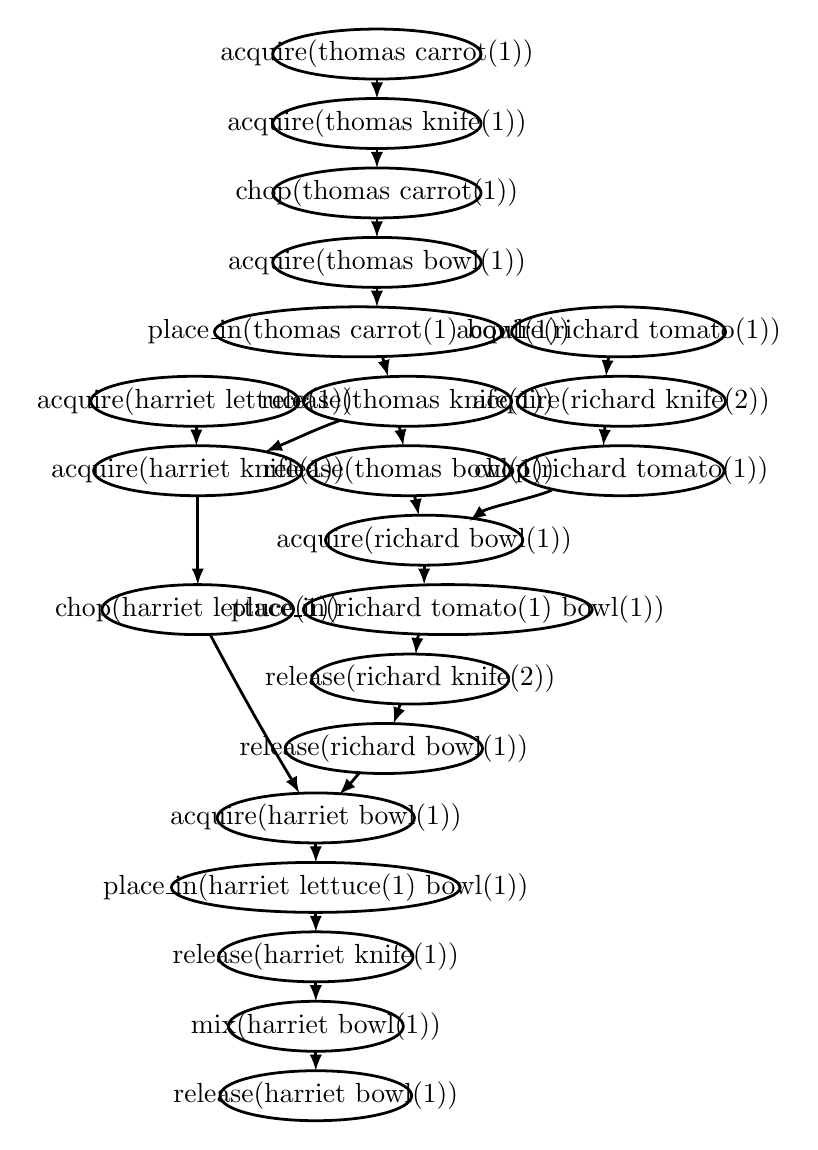
\begin{tikzpicture}[>=latex,join=bevel,scale=0.50]
  \pgfsetlinewidth{1bp}
%
\pgfsetcolor{black}
  % Edge: n0 -> n6
  \draw [->] (196bp,750bp) .. controls (196bp,749bp) and (196bp,748bp)  .. (196bp,736bp);
  % Edge: n2 -> n8
  \draw [->] (363bp,550bp) .. controls (363bp,549bp) and (362bp,547bp)  .. (361bp,536bp);
  % Edge: n6 -> n10
  \draw [->] (196bp,700bp) .. controls (196bp,699bp) and (196bp,698bp)  .. (196bp,686bp);
  % Edge: n8 -> n12
  \draw [->] (360bp,500bp) .. controls (360bp,499bp) and (360bp,497bp)  .. (359bp,486bp);
  % Edge: n10 -> n14
  \draw [->] (196bp,650bp) .. controls (196bp,649bp) and (196bp,648bp)  .. (196bp,636bp);
  % Edge: n14 -> n16
  \draw [->] (196bp,600bp) .. controls (196bp,599bp) and (196bp,598bp)  .. (196bp,586bp);
  % Edge: n16 -> n18
  \draw [->] (200bp,550bp) .. controls (200bp,549bp) and (201bp,547bp)  .. (204bp,536bp);
  % Edge: n18 -> n20
  \draw [->] (212bp,500bp) .. controls (212bp,499bp) and (213bp,497bp)  .. (215bp,486bp);
  % Edge: n18 -> n22
  \draw [->] (169bp,504bp) .. controls (152bp,498bp) and (138bp,491bp)  .. (116bp,482bp);
  % Edge: n4 -> n22
  \draw [->] (66bp,500bp) .. controls (66bp,499bp) and (66bp,498bp)  .. (66bp,486bp);
  % Edge: n20 -> n24
  \draw [->] (223bp,450bp) .. controls (223bp,449bp) and (224bp,447bp)  .. (226bp,436bp);
  % Edge: n12 -> n24
  \draw [->] (322bp,454bp) .. controls (308bp,448bp) and (276bp,442bp)  .. (263bp,432bp);
  % Edge: n22 -> n26
  \draw [->] (67bp,450bp) .. controls (67bp,435bp) and (67bp,413bp)  .. (67bp,386bp);
  % Edge: n24 -> n28
  \draw [->] (230bp,400bp) .. controls (230bp,399bp) and (230bp,398bp)  .. (230bp,386bp);
  % Edge: n28 -> n30
  \draw [->] (226bp,350bp) .. controls (226bp,349bp) and (225bp,347bp)  .. (224bp,336bp);
  % Edge: n30 -> n32
  \draw [->] (213bp,300bp) .. controls (212bp,299bp) and (212bp,297bp)  .. (208bp,286bp);
  % Edge: n32 -> n34
  \draw [->] (184bp,251bp) .. controls (181bp,248bp) and (179bp,245bp)  .. (169bp,235bp);
  % Edge: n26 -> n34
  \draw [->] (76bp,350bp) .. controls (88bp,327bp) and (111bp,285bp)  .. (132bp,250bp) .. controls (133bp,248bp) and (134bp,247bp)  .. (140bp,236bp);
  % Edge: n34 -> n36
  \draw [->] (152bp,200bp) .. controls (152bp,199bp) and (152bp,198bp)  .. (152bp,186bp);
  % Edge: n36 -> n38
  \draw [->] (152bp,150bp) .. controls (152bp,149bp) and (152bp,148bp)  .. (152bp,136bp);
  % Edge: n38 -> n40
  \draw [->] (152bp,100bp) .. controls (152bp,99bp) and (152bp,98bp)  .. (152bp,86bp);
  % Edge: n40 -> n42
  \draw [->] (152bp,50bp) .. controls (152bp,49bp) and (152bp,48bp)  .. (152bp,36bp);
  % Node: n0
\begin{scope}
  \pgfsetstrokecolor{black}
  \draw (196bp,768bp) ellipse (75bp and 18bp);
  \draw (196bp,768bp) node {acquire(thomas carrot(1))};
\end{scope}
  % Node: n2
\begin{scope}
  \pgfsetstrokecolor{black}
  \draw (370bp,568bp) ellipse (77bp and 18bp);
  \draw (370bp,568bp) node {acquire(richard tomato(1))};
\end{scope}
  % Node: n4
\begin{scope}
  \pgfsetstrokecolor{black}
  \draw (65bp,518bp) ellipse (75bp and 18bp);
  \draw (65bp,518bp) node {acquire(harriet lettuce(1))};
\end{scope}
  % Node: n6
\begin{scope}
  \pgfsetstrokecolor{black}
  \draw (196bp,718bp) ellipse (75bp and 18bp);
  \draw (196bp,718bp) node {acquire(thomas knife(1))};
\end{scope}
  % Node: n8
\begin{scope}
  \pgfsetstrokecolor{black}
  \draw (372bp,518bp) ellipse (75bp and 18bp);
  \draw (372bp,518bp) node {acquire(richard knife(2))};
\end{scope}
  % Node: n10
\begin{scope}
  \pgfsetstrokecolor{black}
  \draw (196bp,668bp) ellipse (75bp and 18bp);
  \draw (196bp,668bp) node {chop(thomas carrot(1))};
\end{scope}
  % Node: n12
\begin{scope}
  \pgfsetstrokecolor{black}
  \draw (372bp,468bp) ellipse (74bp and 18bp);
  \draw (372bp,468bp) node {chop(richard tomato(1))};
\end{scope}
  % Node: n14
\begin{scope}
  \pgfsetstrokecolor{black}
  \draw (196bp,618bp) ellipse (75bp and 18bp);
  \draw (196bp,618bp) node {acquire(thomas bowl(1))};
\end{scope}
  % Node: n16
\begin{scope}
  \pgfsetstrokecolor{black}
  \draw (183bp,568bp) ellipse (104bp and 18bp);
  \draw (183bp,568bp) node {place\_in(thomas carrot(1) bowl(1))};
\end{scope}
  % Node: n18
\begin{scope}
  \pgfsetstrokecolor{black}
  \draw (218bp,518bp) ellipse (75bp and 18bp);
  \draw (218bp,518bp) node {release(thomas knife(1))};
\end{scope}
  % Node: n20
\begin{scope}
  \pgfsetstrokecolor{black}
  \draw (219bp,468bp) ellipse (73bp and 18bp);
  \draw (219bp,468bp) node {release(thomas bowl(1))};
\end{scope}
  % Node: n22
\begin{scope}
  \pgfsetstrokecolor{black}
  \draw (67bp,468bp) ellipse (75bp and 18bp);
  \draw (67bp,468bp) node {acquire(harriet knife(1))};
\end{scope}
  % Node: n24
\begin{scope}
  \pgfsetstrokecolor{black}
  \draw (230bp,418bp) ellipse (71bp and 18bp);
  \draw (230bp,418bp) node {acquire(richard bowl(1))};
\end{scope}
  % Node: n26
\begin{scope}
  \pgfsetstrokecolor{black}
  \draw (67bp,368bp) ellipse (69bp and 18bp);
  \draw (67bp,368bp) node {chop(harriet lettuce(1))};
\end{scope}
  % Node: n28
\begin{scope}
  \pgfsetstrokecolor{black}
  \draw (247bp,368bp) ellipse (104bp and 18bp);
  \draw (247bp,368bp) node {place\_in(richard tomato(1) bowl(1))};
\end{scope}
  % Node: n30
\begin{scope}
  \pgfsetstrokecolor{black}
  \draw (220bp,318bp) ellipse (71bp and 18bp);
  \draw (220bp,318bp) node {release(richard knife(2))};
\end{scope}
  % Node: n32
\begin{scope}
  \pgfsetstrokecolor{black}
  \draw (201bp,268bp) ellipse (71bp and 18bp);
  \draw (201bp,268bp) node {release(richard bowl(1))};
\end{scope}
  % Node: n34
\begin{scope}
  \pgfsetstrokecolor{black}
  \draw (152bp,218bp) ellipse (71bp and 18bp);
  \draw (152bp,218bp) node {acquire(harriet bowl(1))};
\end{scope}
  % Node: n36
\begin{scope}
  \pgfsetstrokecolor{black}
  \draw (152bp,168bp) ellipse (104bp and 18bp);
  \draw (152bp,168bp) node {place\_in(harriet lettuce(1) bowl(1))};
\end{scope}
  % Node: n38
\begin{scope}
  \pgfsetstrokecolor{black}
  \draw (152bp,118bp) ellipse (70bp and 18bp);
  \draw (152bp,118bp) node {release(harriet knife(1))};
\end{scope}
  % Node: n40
\begin{scope}
  \pgfsetstrokecolor{black}
  \draw (152bp,68bp) ellipse (63bp and 18bp);
  \draw (152bp,68bp) node {mix(harriet bowl(1))};
\end{scope}
  % Node: n42
\begin{scope}
  \pgfsetstrokecolor{black}
  \draw (152bp,18bp) ellipse (69bp and 18bp);
  \draw (152bp,18bp) node {release(harriet bowl(1))};
\end{scope}
%
\end{tikzpicture}

}}%
%
\end{minipage}}

\caption{ Joint execution for $MakeSalad(bowl(1))$, showing significant concurrency
between agents }


\label{fig:plan-output} 
\end{figure}


We call a sequence of such steps a \emph{run}, which can be converted
to a history by taking just the action and outcome attributes. The
procedure implementing $Trans$ takes a program and a run as input,
returning a new program and new step of execution. As an example consider
the code in figure \ref{fig:trans-code}, implementing the test operator
and the concurrency operator from equation \ref{eqn:trans_conc_orig}.

%
\begin{figure}
\programinput{listings/jointexec/ConGolog.oz}

\caption{Partial code for $Trans$ predicate}


\label{fig:trans-code} 
\end{figure}


Note that whenever the procedure descends through the left side of
a concurrency operator it pushes an 'l' onto the step's {}``thread''
attribute, and each descent through the right side pushes an 'r'.
Two steps can be said to come from different threads as long as neither
{}``thread'' attribute is a prefix of the other.

We say that two steps are \emph{ordered} if any of the following holds:
their action terms are not independent; ones thread is a prefix of
the other; ones action falsifies the test condition associated with
the other. When building a joint execution, ordered steps are forced
to be executed in the order they were generated by the planner, while
unordered steps may be performed independently.


\subsection{Planning Procedure}

The code for planning a joint execution from a given ConGolog program
is shown in figure \ref{fig:planning-code}. The main procedure is
$MakePlan$, a recursive procedure that operates on a list of branches-in-progress
of the form $(D,R,B)$. Here $B$ is a branch in the joint execution
under construction, $D$ is the program remaining to be executed on
that branch, and $R$ is the run of program steps performed on that
branch so far.

%
\begin{figure}
\programinput{listings/jointexec/Planner.oz}

\caption{ Code for main planning loop }


\label{fig:planning-code} 
\end{figure}


%
\begin{figure}
\programinput{listings/jointexec/psearch.oz}

\caption{ Code to run planning procedure in parallel }


\label{fig:parallel-search} 
\end{figure}


Each iteration of the planning loop proceeds as follows. The procedure
$FindOpenBranch$ updates each branch to account for events that were
added since it was last processed (some may have been added automatically
to satisfy restriction (R5)), then searches the list to find a branch
for which $Final(D,R)$ does not hold. If all branches are final,
planning can terminate. Otherwise, the procedure $FindTrans1$ is
called to find a new step of execution for that branch. The action
is inserted into the joint execution, which returns a list of new
branches, one for each possible outcome of the action. Each of these
outcomes is added to the list of branches, and the loop is started
again.

Of particular interest is the procedure $FindTrans1$, which uses
the encapsulated search functionality of Mozart to yield possible
next steps according to an estimate of their potential for concurrency.
The procedure $LP.yieldOrdered$ yields the solutions of the given
search context, sorted using the procedure $CompareSteps$. This procedure
(not shown) gives preference to steps that can be performed concurrently
with as many existing actions as possible.


\subsection{Distributing the Planning Workload}

A primary motivation in using Mozart/Oz for our implementation is
its strong support for distributed logic programming. Utilizing Mozart's
parallel search functionality \citep{Schulte00constraint_services},
the planning workload can be transparently distributed between the
agents in the team.

Figure \ref{fig:parallel-search} shows the necessary code, which
should be executed by one of the agents. The planning procedure is
encapsulated in a \emph{functor}, a portable code object. A parallel
search object is then created, which uses an ssh connection to spawn
remote computations on each of the three agents (identified by their
DNS names). The object is asked to provide a single solution, which
is then written to a file in the graphviz 'dot' format for display
(resulting in figure \ref{fig:plan-output}).

For the simple example shown in this paper, parallel plan search does
not demonstrate a significant time saving since almost no backtracking
is required to reach a solution. For more difficult problems, significant
gains can be expected.


\section{Discussion\label{sec:JointExec:Discussion}}

In this section we have defined a \emph{joint execution} as a prime
event structure with some additional restrictions. We contend that
such structures are highly suitable for planning the actions to be
performed by a team in service of some shared task, such as executing
a shared Golog program.

On one hand, joint executions are restricted enough to be practical
for such use. Prime event structures are purely reactive (equivalent
to a kind of finite automaton) and can be executed by the agents without
further deliberation. They are restricted to ensure that whenever
an agent is required to perform an action, it is able to determine
this using only its local information. Each branch of execution can
be easily converted into a situation term for the purposes of reasoning,
and can be extended one action at a time.

Joint executions are also significantly more flexible than previous
approaches. They allow independent actions to be performed without
synchronization, in any order. The agents need never know precisely
what actions have been executed, only those that enable them to perform
their next action. Synchronization is automatically achieved when
required by explicitly reasoning about what actions each agent can
observe, rather than requiring that all actions be public.

To demonstrate the utility of these structures, we have implemented
an interpreter for multi-agent ConGolog programs that produces joint
executions as its output. In the next section, we highlight the key
aspects of our implementation and give an example of the output it
produces.

An alternate approach to the problem of partial observability is the
language TeamGolog developed in \citep{farinelli07team_golog}, where
agents explicitly synchronize through communication and a shared state.
By contrast, our approach constructs synchronization implicitly by
reasoning about the actions that can be observed by each agent. This
has the advantage of requiring no changes to the form or semantics
of the agents' control program, but the disadvantage that joint execution
construction may fail if too many actions are unobservable. It would
be interesting to combine these approaches by automatically incorporating
explicit communication when implicit synchronization is not possible.

There is, of course, an extensive body of work on partial-order planning
in the context of goal-based planning. Unsurprisingly, the joint execution
structure we develop here has deep similarities to the structures
used in conditional partial-order planners such as \citep{peot92conditional_nonlinear}.
It is, however, intentionally specific to the situation calculus.
We make no use of many concepts common in partial-order goal-based
planning (causal links, threats, conflicts, etc) because we do not
deal explicitly with goals, but with steps generated by an underlying
transition semantics. Our approach can be considered roughly equivalent
to \emph{deordering} of a totally-ordered plan as described in \citep{backstrom99reordering},
except performed during plan construction rather than as a post-processing
step.

loops: \citep{levesque96what_is_planning,levesque05planning_with_loops}

can't represent actions that {*}need{*} to be performed concurrently
- but should be a trivial addition.

don't use explicit mental attitiudes, mutual beliefs etc. JE's more
akin to recpies in SharedPlans. Assume agents all have the common
goal of executing the given shared program. But it could be used as
part of larger system.


\subsubsection{Online Execution}

In this section we have defined a \emph{joint execution} as a prime
event structure with some additional restrictions. We contend that
such structures are highly suitable for planning the actions to be
performed by a team in service of some shared task, such as executing
a shared Golog program.

On one hand, joint executions are restricted enough to be practical
for such use. Prime event structures are purely reactive (equivalent
to a kind of finite automaton) and can be executed by the agents without
further deliberation. They are restricted to ensure that whenever
an agent is required to perform an action, it is able to determine
this using only its local information. Each branch of execution can
be easily converted into a situation term for the purposes of reasoning,
and can be extended one action at a time.

Joint executions are also significantly more flexible than previous
approaches. They allow independent actions to be performed without
synchronization, in any order. The agents need never know precisely
what actions have been executed, only those that enable them to perform
their next action. Synchronization is automatically achieved when
required by explicitly reasoning about what actions each agent can
observe, rather than requiring that all actions be public.

To demonstrate the utility of these structures, we have implemented
an interpreter for multi-agent ConGolog programs that produces joint
executions as its output. In the next section, we highlight the key
aspects of our implementation and give an example of the output it
produces.

Capturing \emph{online} execution in an syncrhonous domain is less
straightforward, as it is difficult to single-step an execution in
a partially-observable setting. Consider, for example, a program whose
next step is a sensing action to be performed by some agent. Before
the action is performed, the joint execution will contain one branch
for each possible sensing outcome. Once the action is performed, that
particular agent will know which leaf corresponds to the actual world,
and can avoid trying to plan a next step for any of the other leaves.

However, its team-mates will \emph{not} know the outcome of the sensing
action, so from their perspective any of the potential leaves might
be the real state of the world. They are therefore forced to plan
a next step in each one of those leaves. But they must also account
for what they think that the team-mate things..etc etc TODO find a
way to explain this!

The difficulty here is due to the well-known correspondance between
coordination and common knowledge - the agents must develop a plan
extending every leaf of the joint execution unless it is common knowledge
that that leaf is not legal. Reasoning about common knowledge is very
difficult and we want to avoid it if we can.

